% !TEX encoding = UTF-8 Unicode
\documentclass{beamer}
%\documentclass[handout]{beamer}

\mode<presentation>
{% AnnArbor
%\usetheme{AnnArbor}
  %\usetheme{Boadilla}
  \usetheme{CambridgeUS}
 %\usetheme{Madrid}
  \setbeamercovered{transparent}
}

\usepackage{fontspec,xltxtra,xunicode,moreverb}

\usepackage[french]{babel}
% \usepackage{beamerthemesplit} // Activate for custom appearance

%% No navigation symbol.
\setbeamertemplate{navigation symbols}{}
\beamertemplatenavigationsymbolsempty

%\setbeameroption{hide notes}

\newcommand{\mypause}{\pause}
% \newcommand{\mypause}{~}

\newcommand{\elvrm}{\rm}
\newcommand{\fivrm}{\rm}
\newcommand{\sixrm}{\rm}
\newcommand{\sevrm}{\rm}
\newcommand{\egtrm}{\rm}
\newcommand{\ninrm}{\rm}
\newcommand{\tenrm}{\rm}
\newcommand{\twlrm}{\rm}
\newcommand{\frtnrm}{\rm}
\newcommand{\svtnrm}{\rm}
\newcommand{\twtyrm}{\rm}
\newcommand{\twfvrm}{\rm}

\newcommand{\ex}{{\bf Exemple}}
\newcommand{\afor}{\bf for}
\newcommand{\ato}{\bf to}
\newcommand{\ado}{\bf do}
\newcommand{\aendo}{\bf endo}
\newcommand{\esp}{\hspace{0.5cm}}

\newcommand{\sal}{\sum_i \mu_i}
\newcommand{\sbet}{\sum_j \nu_j}
\newcommand{\If}{\mbox{\bf if }}
\newcommand{\Then}{\,\mbox{\bf then }}
\newcommand{\titre}[1]{\title{{{\color{red} \large \bf #1}}}}

% Needed for course 2. 
\newcommand{\Zn}{{\bf Z}^n}
\newcommand{\Z}{{\bf Z}}
\newcommand{\N}{{\bf N}}
\newcommand{\Np}{{\bf N}^p}

\newcommand{\alfa}{\textsc{alpha}}
\newcommand{\alfacase}{\mbox{\bf case}}
\newcommand{\alfaesac}{\mbox{\bf esac}}
\newcommand{\zset}{\mathbb{Z}}

\newcommand{\sys}{{\bf system}}
\newcommand{\real}{{\bf real}}
\newcommand{\of}{{\bf of}}
\newcommand{\lett}{{\bf let}}
\newcommand{\tel}{{\bf tel}}
\newcommand{\returns}{{\bf returns}}
\newcommand{\boolean}{{\bf boolean}}
\newcommand{\true}{{\bf true}}
\newcommand{\false}{{\bf false}}

\newcommand{\pomme}{\texttt{cmd}}
\newcommand{\alalign}{{$\hookleftarrow$}}

\newcommand{\pyth}{{\sc python}}
\newcommand{\prog}[1]{\alert{\texttt{#1}}}

\title{Introduction à l'Informatique}
% \author{Patrice Quinton}
\author{Lilian Besson}
\date{2020\\Version du \today}

\institute% (optional, but mostly needed)
{ENS Rennes}

\date%[\today] % (optional, should be abbreviation of conference name)
[Info - DEM - 2020]{Initiation à l'Informatique -- DEM -- 2020\\Module 1}%\logo{
\includegraphics[height=0.5cm]{logoENS.pdf}}

\pgfdeclareimage[height=0.5cm]{adb-logo}{logoENS.pdf}
\logo{\pgfuseimage{adb-logo}}

% Delete this, if you do not want the table of contents to pop up at
% the beginning of each subsection:
\AtBeginSection[]
{
  \begin{frame}<beamer>
    \frametitle{Outline}
%    \tableofcontents[currentsection,currentsubsection]
\tableofcontents[currentsection,currentsubsection,hideallsubsections]
  \end{frame}
}

\begin{document}

\frame{\titlepage}

\section[Outline]{}
\frame{\tableofcontents}

\section{Introduction}


\frame
{
  \frametitle{Qu'est-ce qu'on va faire?}

  \begin{itemize}
  \item Découvrir ce qu'est un \prog{algorithme}\mypause{}
  \item Découvrir le principe de fonctionnement d'un \prog{ordinateur}\mypause{}
  \item Apprendre un langage répandu, utile, gratuit (un {\em logiciel libre})\mypause{}
  \item Découvrir certains aspects du \prog{monde numérique}, et réfléchir à ses conséquences\mypause{}
  \item S'amuser... (j'espère)\mypause{}
  \item Cela va durer 12h (6 séances de 2h)\mypause{}
  \end{itemize}
}



\frame
{
  \frametitle{Objectif}

  \begin{itemize}
  \item Vous donner des \prog{points de référence} sur ce qu'un ordinateur peut faire\mypause{}
  \item Pour cela, il est nécessaire de \prog{programmer} un peu\mypause{}
  \item À la fin de ce cours, vous aurez acquis un certain nombre de \prog{notions fondamentales}
  qui vous serviront certainement (un jour ou l'autre...)\mypause{}
  \item Le langage choisi, \prog{\pyth{}}, est un logiciel libre, qui peut être utilisé sur
  n'importe quel ordinateur\mypause{}
  \item Je reprends un cours créé et donné pendant trois ans par Patrice Quinton
  \item \prog{Première} année de cette expérience (pour moi) : votre avis m'intéresse !
  \end{itemize}
}

\frame
{
  \frametitle{Méthode}

  \begin{itemize}
  \item On privilégie la \prog{pratique}: on sera toujours devant un ordinateur\mypause{}
  \item Je présente une \prog{notion} (avec des projections dont vous aurez la copie)\mypause{}
  \item La page web du cours est \texttt{perso.crans.org/besson/teach/intro\_num\_DEM\_2020/} : \textbf{notez la}
  \item Vous pratiquez en \prog{binôme}\mypause{}
  \item On fait une \prog{pause} toutes les heures\mypause{}
  \item Je vous donnerai à chaque fin de cours un tout petit travail personnel de 5mn,
  que vous faites... ou pas\mypause{}
  \item Vous pouvez travailler \prog{ensemble}, copier sur le-la voisin-e\mypause{}
  \item L'assiduité est \prog{obligatoire}\mypause{}
  \item L'évaluation se fera en \prog{auto-évaluation} au dernier cours 6\mypause{}
  \end{itemize}
}

\frame
{
  \frametitle{Des petites histoires}
À la fin d'une séance, je prendrai 5-10mn pour vous raconter une {\em petite histoire}, développer
un petit sujet (qui pourra donner lieu à débat). Voici une liste des idées que j'ai:
  \begin{itemize}
  \item Ada Lovelace, la première programmeuse
  \item Alan Turing, un informaticien sans ordinateur
  \item Grace Hoper, l'inventrice du premier langage de programmation
  % \item Les grammaires de Noam Chomsky
  \item 50 ans d'informatique et de programmeur-se-s : de la mission Apollo à la première image d'un trou noir
  \item Comment un ordinateur reconnaît-il la parole
  \item Comment un ordinateur identifie-t-il une photo
  \item Comment fait-on pour fabriquer un circuit intégré
  % \item Logique et droit
  \item Intelligence artificielle...
  \end{itemize}
  
Si vous en avez d'autres idées, et que je suis en mesure de les traiter, n'hésitez pas !
}


\frame
{
  \frametitle{Remarque importante}

Je ne connais pas votre niveau en informatique. \mypause{}

J'ai donc supposé que vous ne savez pas grand chose. \mypause{}

\hspace{10pt}

Si je vais trop vite, dites-le moi ! \mypause{}

Si je vais (vraiment) trop lentement, dites-le moi aussi ! \mypause{}

\hspace{10pt}

Si vous êtes déjà vraiment très bon-ne en informatique, aidez les autres !
}

\section{Mon premier algorithme : informatique {\em débranchée}}
\frame
{
\frametitle{Le crêpier psycho-rigide}
\begin{block}{Le problème}
\mypause{}
Tous les soirs, Yann le crêpier compte les crêpes qui lui restent, 
et les emballe soigneusement dans du papier cellophane pour les
protéger. 
\mypause{}

Mais avant, il doit les ranger par taille, les plus grandes
en dessous.
\mypause{}

Pour ranger ses crêpes sans les abimer, il peut 
seulement glisser une spatule sous une pile de crêpes, et
hop, retourner la pile.

\mypause{}
Sa fille, Maïwenn, qui est une algorithmicienne avertie, lui a inventé une
méthode systématique pour ranger ses crêpes par taille.

\textbf{À vous de trouver sa méthode !}

\end{block}
}

% \frame
% {
% \frametitle{Le crêpier psycho-rigide}
% \begin{block}{Comment on procède}
% \begin{enumerate}
% \item
% Vous vous mettez par groupes de 3, et vous réfléchissez à 
% la méthode, avec le simulateur de crêpes que je vais vous donner
% \mypause{}
% \item
% Quand vous avez trouvé une méthode, l'un-e d'entre vous 
% va jouer le rôle de l'ordinateur à qui on donne des ordres
% (un robot), un-e autre va donner les ordres, et les deux
% autres vont contrôler que tout se passe bien
% \mypause{}
% \item
% Même chose, mais celui-celle qui donne les ordres
% ne regarde plus la pile de crêpes.\mypause{}
% \item
% Même chose, mais il y a deux "robots" au lieu d'un et on donne
% les ordres pour les deux (il faut se mettre par groupe de 6)
% \end{enumerate}
% \end{block}
% }

\frame
{
\frametitle{Le crêpier psycho-rigide}
\begin{block}{Comment on procède}
\begin{enumerate}
\item
Sans la COVID, on ferait une activité d'informatique débranchée par groupe... à la place...
\mypause{}
\item
Vous vous mettez par binôme, et vous réfléchissez à la méthode,
\mypause{}
\item
Quand vous avez trouvé une méthode, l'un-e d'entre vous
va jouer le rôle de l'ordinateur à qui on donne des ordres
(un robot), un-e autre va donner les ordres, et les deux
autres vont contrôler que tout se passe bien,
\mypause{}
\item
Quand tout le monde a trouvé, je montre la solution.
% \item
% Même chose, mais celui-celle qui donne les ordres
% ne regarde plus la pile de crêpes.\mypause{}
% \item
% Même chose, mais il y a deux "robots" au lieu d'un et on donne les ordres pour les deux (il faut se mettre par groupe de 6)
\end{enumerate}
\end{block}
}

\frame{
\frametitle{Les algorithmes}
\begin{itemize}
  \item Ce que vous avez fait s'appelle un \alert{algorithme.}\mypause{}

  \item Exemple de représentation graphique d'un algorithme (pas étudiée dans ce cours)
  \begin{center}
    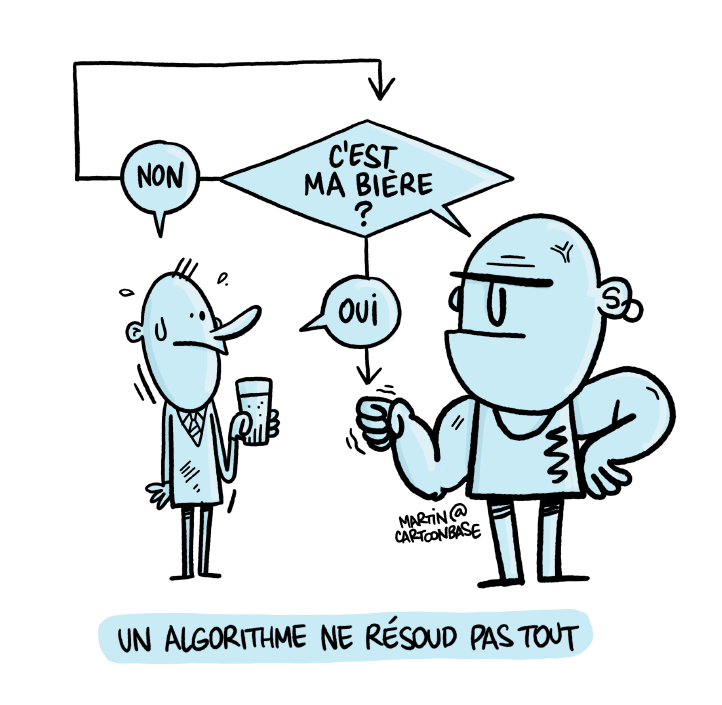
\includegraphics[height=150pt]{un-algorithme-ne-resoud-pas-tout.png}
  \end{center}
\end{itemize}
  }

\frame{
\frametitle{Un algorithme}
\begin{itemize}

\item C'est un \alert{procédé systématique} qui permet de résoudre un 
problème \mypause{}
\item Pour résoudre un problème informatique, on respecte en général la méthode suivante:
\begin{itemize}
\item On commence par \alert{inventer} un algorithme\mypause{}
\item On s'assure qu'il est \alert{correct}, c'est-à-dire, qu'il fait bien ce qu'on souhaite, 
et qu'il se termine (tout cela, c'est difficile) \mypause{}
\item Puis on le \alert{programme} (on dit aussi, on le code) et on le met au point (on 
le débogue, on le dévermine) \mypause{}
\item Puis on le \alert{teste} (c'est long et fastidieux) ou on le prouve (c'est très très difficile) \mypause{}
\item Enfin, on le \alert{documente} \mypause{}
\item Parfois, on le vend, souvent, on l'oublie, ou on le donne
\end{itemize}
\end{itemize}\mypause{}

Ce qu'on vient de faire s'appelle de {\em l'informatique débranchée}. (Le crêpier psycho-rigide
est dû à Martin Quinson et Jean-Christophe Bach)
}

% \section{Petit historique sur les algorithmes}
\frame
{
  \frametitle{Deux définitions d'un algorithme}

  \footnotesize{
  \begin{itemize}
    \item
    D'après Wikipédia : ``Un algorithme est une suite finie et non ambiguë d'opérations ou d'instructions permettant de résoudre une classe de problèmes''.

    \item
    D'après Gérard Berry : ``Un algorithme, c'est tout simplement une façon de décrire dans ses moindres détails comment procéder pour faire quelque chose. Il se trouve que beaucoup d'actions mécaniques, toutes probablement, se prêtent bien à une telle décortication. Le but est d'évacuer la pensée du calcul, afin de le rendre exécutable par une machine numérique (ordinateur…).''

    \item
    Le mot \textit{algorithme} vient du nom d'un mathématicien perse du IXe siècle, \textit{Al-Khwârizmî}.

    \item
    Les algorithmes sont aussi vieux que l'écriture : par exemples
    \begin{itemize}
      \item pour calculer la division par les Babyloniens, -2500 av JC
      \item calcul de racines carrés par les Babyloniens, -1800 av JC
      \item calcul de PGCD par Euclide, -600 av JC
    \end{itemize}

    \item
    Exemples non numériques : recettes de cuisine, plans de bataille, traitement d'images / textes / sons, etc
  \end{itemize}
  }
}

\frame{
  \frametitle{Plus vieil exemple connu : tablette en argile YBC 7289}

  \begin{center}
    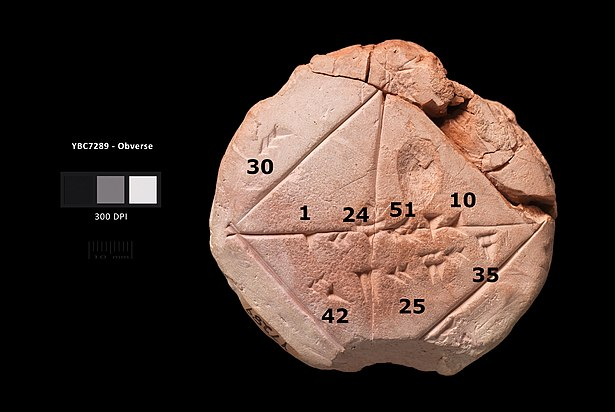
\includegraphics {615px-YBC-7289-OBV-labeled.jpg}
  \end{center}

  Tablette estimée à -1800 / -1600 av JC, donnant une valeur approchée de la longueur de la diagonale d'un carré unité, $\sqrt{2}$, à six chiffres décimaux après la virgule :

  En base $16$, $1;24,51,10$ représente le nombre $305470/216000 \simeq 1.414213$.

  Les Babyloniens avaient une méthode efficace, systématique, pour faire ce genre de calculs.
  % (cas particulier de la méthode de Newton pour résoudre $f(x)=0$, 3000 ans avant Newton)
}

% \frame{
%   \frametitle{Représentation de l'algorithme d'Euclide}

%   \vspace*{250pt}
%   \hspace*{75pt}
%   % \includegraphics[height=15pt]{455px-Euclid_flowchart.svg.png}
%   \includegraphics[height=15pt]{455px-Euclid_flowchart.png}
% }

\frame{
  \frametitle{Pause}

  Pause de 5 minutes.
}

\section{Votre environnement de travail}
\frame
{
  \frametitle{Votre environnement de travail}
{\footnotesize
  \begin{itemize}
  \item Je suppose que vous êtes connecté (on dit aussi {\em loggé} -- prononcer logué.) \mypause{}
  \item Trouvez un terminal. 
  \begin{itemize}
  \item Sous MacOS, il faut aller chercher dans \prog{Applications/Utilitaires/Terminal.app}\mypause{}.
  \item Sous Windows, rechercher un programme qui s'appelle \prog{Invite de commandes}\mypause{}
  \end{itemize}\mypause{}
  \item On peut placer l'icône de l'application dans le {\em dock} pour l'avoir à porté de main\mypause{}
  \item Double-cliquez sur l'icône de l'application pour la lancer\mypause{}
  \item Placez la souris dedans, et tapez \prog{pwd} (abréviation de \prog{print working
  directory})\mypause
  \item Vous devez avoir en réponse quelque chose du genre
  \texttt{/home/votrenom}. C'est le nom de votre {\em répertoire courant}.\mypause{}
  \item La commande \prog{ls} (\prog{dir} sous Windows) vous permet de lister tous les fichiers de votre répertoire
  courant\mypause{}
  \item Si vous cherchez des détails sur une commande, utilisez la commande \prog{man com}
  (mais c'est en anglais, et souvent (très) long)
  \end{itemize}
}
}
\frame
{
  \frametitle{Gérer son environnement de travail}
 Avec le terminal, vous êtes en relation directe avec le {\em système d'exploitation}
 de votre ordinateur (Ubuntu/Linux, ou Windows, ou Mac OS)\mypause{}
{\footnotesize
  \begin{itemize}
  \item la commande \prog{pwd} ({\color{blue} dir}) exécutée dans votre terminal vous indique dans
  quel répertoire (dossier) vous vous trouvez, le répertoire \prog{courant} \mypause{}
  \item les commandes suivantes sont utiles
  \begin{itemize}
  \item \prog{ls}: lister les fichiers (et répertoires) du répertoire courant  ({\color{blue} dir} sous Windows)\mypause{}
  \item \prog{ls -l}: comme ls, mais avec plein d'informations\mypause{}
  \item \prog{mkdir d}: crée un répertoire appelé \prog{d} dans le répertoire courant (mkdir vient de make directory) \mypause{}
  \item \prog{cd d}: faire que d devient le répertoire courant \mypause{}
  \item \prog{cp f1 f2} ({\color{blue} copy f1 f2}): copier le fichier (ou le répertoire) f1 sous le nom f2 \mypause{}
  \item \prog{mv f1 f2} ({\color{blue} rename f1 f2}): déplacer le fichier (ou le répertoire) f1 en f2 (\prog{move})\mypause{}
  \item \prog{rm f1} ({\color{blue} del f1}): supprimer le fichier f1 
\end{itemize}
  \end{itemize}\mypause{}
}
}

\frame
{
  \frametitle{Le nommage des fichiers (et des répertoires)}
{\footnotesize
  \begin{itemize}
  \item le nom {\em relatif} d'un fichier est donné par rapport au répertoire courant. 
 Lorsqu'on exécute \prog{ls}, on obtient la liste des noms relatifs des fichiers dans 
 le répertoire courant
   \mypause{}
  \item le nom de votre répertoire personnel ({\em home directory}) est \prog{/home/votreNom}
({\color{blue} C:$\backslash$} sous Windows)
\mypause{}
  \item le nom {\em absolu} d'un fichier \prog{f} est le nom du répertoire où il se situe, auquel
  on ajoute \prog{/f}. Donc, si \prog{f} est dans le répertoire personnel, son nom absolu
  est \prog{/home/votreNom/f} ({\color{blue} C:$\backslash$f} sous Windows)\mypause{}
  \item le nom relatif du répertoire courant est aussi noté \prog{.} \mypause
  \item le nom relatif de l'unique répertoire qui contient le répertoire courant est aussi noté \prog{..}
\end{itemize}\mypause{}
}
}

\frame
{
\frametitle{La métaphore des fenêtres}
{\footnotesize
\begin{itemize}
\item La vision que nous donne l'écran du contenu de l'ordinateur est une \prog{métaphore} 
destinée à nous simplifier la vie \mypause{}
\item Une \prog{fenêtre} représente le contenu d'un répertoire \mypause{}
\item Le curseur de la souris permet de \prog{désigner} un fichier ou un répertoire d'une fenêtre \mypause{}
\item Le simple fait de déplacer la souris sur une nouvelle fenêtre a le même effet que 
la commande \prog{cd} \mypause{}
\item Si je double-clique sur un dossier, il s'ouvre et \prog{j'entre} dans le répertoire qu'il représente.
C'est aussi une autre façon d'effectuer la commande \prog{cd}
\mypause{}
\item Mais... si cette métaphore est très pratique (conviviale), {\em elle ne permet pas de 
programmer les déplacements de fichiers, etc.} comme le peuvent les commandes \mypause{}
\item Sur chaque système, il existe un langage permettant les manipulations de fichiers: 
qu'on appelle souvent un \prog{langage de script}, ou un \prog{shell}, ou un \prog{langage de commandes}
\end{itemize}
}
}

\frame
{
\frametitle{Exercice}
{\footnotesize
\begin{enumerate}
\item Ouvrez le terminal\mypause{}
\item Dans quel répertoire vous trouvez-vous?\mypause{}
\item Créez un nouveau répertoire appelé \texttt{Cours-Info}\mypause{}
\item Allez dans ce répertoire\mypause{}
\item Avec votre éditeur de texte (Word, LibreOffice, ...), créez un fichier, et
sauvez-le dans ce répertoire sous le nom \prog{essai}\mypause{}
\item Faites une copie de ce fichier sous un autre nom (\prog{essai1})\mypause{}
\end{enumerate}
}
}


\section{La petite histoire: Ada Lovelace}

\frame{
\frametitle{Ada Lovelace}
{\footnotesize
\begin{itemize}
\item Née en 1815, fille de Lord Byron (le poète romantique) et d'Anabelle Milanke, 
mathématicienne
\item Elle fait connaissance à 17 ans de Charles Babbage, considéré comme l'inventeur
du premier ordinateur, la \prog{machine à différences}
\item Elle traduit, en collaboration avec Babbage, un mémoire écrit en Français décrivant
le fonctionnement de sa machine
\item Ce faisant, elle écrit des programmes, invente le \prog{branchement}, la \prog{boucle},
et elle est la première à comprendre, 100 ans avant Turing, l'universalité de l'ordinateur
% \item Mais elle restera quasiment inconnue
\item Elle meurt à 36 ans d'un cancer
\item Voir \texttt{http://binaire.blog.lemonde.fr/2015/03/07/la-visionnaire-ada-lovelace/} (rédigé par Anne-Marie Kermarrec, ancienne chercheuse INRIA à Rennes)
\end{itemize}
}
}


\section{A faire pour le cours suivant : installer Python}

\frame{
\frametitle{Installer Python sur votre ordinateur personnel}
{\footnotesize
D'ici le cours suivant (vendredi 18 septembre, 10h-12h, même salle Téléprésence),\\
je vous demande d'\textbf{installer Python sur votre ordinateur personnel}.
\begin{itemize}
\item Sur Mac OS et Linux, c'est normalement déjà installé par défaut
\item Sur Windows, ça ne l'est pas
\item Il faut l'installer à partir de \texttt{www.python.org/downloads/}
\mypause{}
\item Si besoin : un bon tutoriel vidéo : \texttt{www.youtube.com/watch?v=IS117\_uXZKE}
\mypause{}
\item Essayez de lancer Python et son éditeur de texte Idle.\\
  Si besoin : un bon tutoriel vidéo : \texttt{www.youtube.com/watch?v=QtUxL52VPtA}
% \item Si ça ne fonctionne pas, essayez à partir de \texttt{www.anaconda.com/products/individual}
\item (la chaîne YouTube "Python au lycée" donne de bons tutoriels \texttt{www.youtube.com/channel/UC6PiFyqBiUjiJ7Q3DRSW2Wg})
\end{itemize}
}
}





\end{document}
